%%%%%%%%%%%%%%%%%%%%%%%%%%%%%%%%%%%%%%%%%%%%%%%%%%%%%%%%%%%%%%%%
%%%%%%%%%%%%%%%%%%%%%%%%%%% Metadata %%%%%%%%%%%%%%%%%%%%%%%%%%%
%%%%%%%%%%%%%%%%%%%%%%%%%%%%%%%%%%%%%%%%%%%%%%%%%%%%%%%%%%%%%%%%
\documentclass{Axon}

\title{Discrete Mathematics and its Applications, 8th Edition - Chapter 1 The Foundations: Logic and Proofs - Section 1.3 Propositional Equivalences - Subsection 1.3.6 Applications of Satisfiability}

\authors{
    \addauthor{Jeffrey G. Lind III}{jeffrey@jeffreylind.dev}
}

\addbibresource{Bibliography.bib}
%%%%%%%%%%%%%%%%%%%%%%%%%%%%%%%%%%%%%%%%%%%%%%%%%%%%%%%%%%%%%%%%
%%%%%%%%%%%%%%%%%%%%%%%%%%%%% Paper %%%%%%%%%%%%%%%%%%%%%%%%%%%%
%%%%%%%%%%%%%%%%%%%%%%%%%%%%%%%%%%%%%%%%%%%%%%%%%%%%%%%%%%%%%%%%
\begin{document}
\maketitle
\makeauthor
%%%%%%%%%%%%%%%%%%%%%%%%%%%%%%%%%%%%%%%%%%%%%%%%%%%%%%%%%%%%%%%%
%%%%%%%%%%%%%%%%%%%%%%%%%%% Abstract %%%%%%%%%%%%%%%%%%%%%%%%%%%
%%%%%%%%%%%%%%%%%%%%%%%%%%%%%%%%%%%%%%%%%%%%%%%%%%%%%%%%%%%%%%%%
\begin{abstract}
Notes on Discrete Mathematics and its Applications, 8th Edition - Chapter 1 The Foundations: Logic and Proofs - Section 1.3 Propositional Equivalences - Subsection 1.3.6 Applications of Satisfiability \cite{Rosen}.
\end{abstract}
%%%%%%%%%%%%%%%%%%%%%%%%%%%%%%%%%%%%%%%%%%%%%%%%%%%%%%%%%%%%%%%%
%%%%%%%%%%%%%%%%%%%%%%%%%%% Section 1 %%%%%%%%%%%%%%%%%%%%%%%%%%
%%%%%%%%%%%%%%%%%%%%%%%%%%%%%%%%%%%%%%%%%%%%%%%%%%%%%%%%%%%%%%%%
\section{Introduction}
Many problems, in diverse areas such as robotics, software testing, artificial intelligence planning, computer-aided design, machine vision, integrated circuit design, scheduling, computer networking, and genetics, can be modeled in terms of propositional satisfiability. Although most applications are quite complex and beyond the scope of this book, we can illustrate how two puzzles can be modeled as satisfiability problems.

\begin{example}\label{Example: 10}
    \textbf{The \textit{n}-Queens problem}
    The \(n\)-queens problem asks for a placement of \(n\) queens on an \(n \times n\) chessboard so that no queen can attack another queen. This means that no two queens can be placed in the same row, in the same column, or on the same diagonal. We display a solution to the eight-queens problem in Figure \ref{Figure: 1}. (The eight-queens problem dates back to 1848 when it was proposed by Max Bezzel and was completely solved by Franz Nauck in 1850. We will return to the \(n\)-queens problem in Section 11.4.)

    To model the \(n\)-queens problem as a satisfiability problem, we introduce \(n^2\) variables, \(p(i, j)\) for \(i = 1, 2, \ldots, n\) and \(j = 1, 2, \ldots, n\). For a given placement of a queens on the chessboard, \(p(i, j)\) is true when there is a queen on the square in the \(i\)th row and \(j\)th column, and is false otherwise. Note that squares \((i, j)\) and \((i', j')\) are on the same diagonal if either \(i + j = i' + j'\) or \(i - i' = j - j'\). In the chessboard in Figure \ref{Figure: 1}, \(p(6, 2)\) and \(p(2, 1)\) are true, while \(p(3, 4)\) and \(p(5, 4)\) are false.

    For no two of the \(n\) queens to be in the same row, there must be one queen in each row. We can show that there is one queen in each row by verifying that every row contains at least one queen and that everyone row contains at most one queen. We first note that \(\bigvee_{j = 1} ^ n p(i, j)\) asserts that row \(i\) contains at least one queen, and
    \begin{equation*}
        Q_1 = \bigwedge_{i = 1}^n \bigvee_{j = 1}^n p(i, j)
    \end{equation*}
    asserts that every row contains at least one queen.

    For every row to include at most one queen, it must be the case that \(p(i, j)\) and \(p(i, k)\) are not both true for integers \(j\) and \(k\) with \(1 \leq j < k \leq n\). Observe that \(\lnot p(i, j) \lor \lnot p(i, k)\) asserts that at least one of \(\lnot p(i, j)\) and \(\lnot p(i, k)\) is true, which means that at least one of \(p(i, j)\) and \(p(i, k)\) is false. So, to check that there is at most one queen in each row, we assert
    \begin{equation*}
        Q_2 = \bigwedge_{i = 1}^n \bigwedge_{j = 1}^{n - 1} \bigwedge_{k = j + 1}^n (\lnot p(i, j) \lor \lnot p(i, k)).
    \end{equation*}

    To assert that no column contains more than one queen, we assert that
    \begin{equation*}
        Q_3 = \bigwedge_{j = 1}^n \bigwedge_{i = 1}^{n - 1} \bigwedge_{k = i + 1}^n (\lnot p(i, j) \lor \lnot p(k, j)).
    \end{equation*}
    
    \begin{figure}[ht]
        \centering
        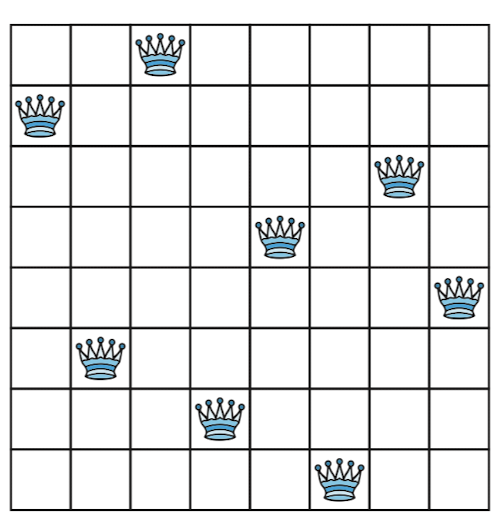
\includegraphics[width=0.25\linewidth]{Discrete Mathematics and its Applications, 8th Edition/Chapter 1 Logic and Proofs/Section 1.3 Propositional Equivalences/Figure 1.png}
        \caption{}
        \label{Figure: 1}
    \end{figure}
    
    (This assertion, together with the previous assertion that every row contains a queen, implies that every column contains a queen.)
    
    To assert that no diagonal contains two queens, we assert
    \begin{equation*}
        Q_4 = \bigwedge_{i = 2}^n \bigwedge_{j = 1}^{n - 1} \bigwedge_{k = 1}^{\min(i - 1, n - j)} (\lnot p(i, j) \lor \lnot p(i - k, k + j))
    \end{equation*}
    and
    \begin{equation*}
        Q_5 = \bigwedge_{i = 1}^{n - 1} \bigwedge_{j = 1}^{n - 1} \bigwedge_{k = 1}^{\min(n - i, n - j)} (\lnot p(i, j) \lor \lnot p(i + k, j + k)).
    \end{equation*}
    
    The innermost conjunction in \(Q_4\) and in \(Q_5\)for a pair \((i, j)\) runs through the positions on a diagonal that begin at \((i, j)\) and runs rightward along this diagonal. The upper limits on these innermost conjunctions identify the last cell in the board on each diagonal.
    
    Putting this all together, we find that the solution of the \(n\)-queens problem are given by the assignments of truth values to the variables \(p(i, j)\), \(i = 1, 2, \ldots, n\) and \(j = 1, 2, \ldots, n\) that make
    \begin{equation*}
        Q = Q_1 \land Q_2 \land Q_3 \land Q_4 \land Q_5
    \end{equation*}
    true.
    
    Using this and other approaches, the number of ways \(n\) queens can be placed on a chessboard so that no queen can attack another has been computed for \(n \leq 27\). When \(n = 8\) there are \(92\) such placements, while for \(n = 16\) this number grows to \(14,772,512\). (See the OEIS discussed in Section 2.4 for details.)
\end{example}

\begin{example}
    \textbf{Sudoku} Sudoku puzzles are constructed using a \(9 \times 9\) grid made up of nine \(3 \times 3\) subgrids, known as \textbf{blocks}, as shown in Figure \ref{Figure: 2}.

    \begin{figure}[ht]
    \centering
    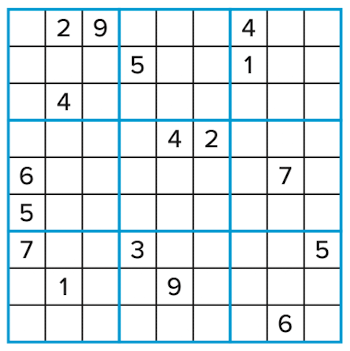
\includegraphics[width=0.25\linewidth]{Discrete Mathematics and its Applications, 8th Edition/Chapter 1 Logic and Proofs/Section 1.3 Propositional Equivalences/Figure 2.png}
    \caption{\textbf{A \(9 \times 9\) Sudoku puzzle.}}
    \label{Figure: 2}
    \end{figure}

    For each puzzle, some of the \(81\) cells, called \textbf{givens}, are assigned one of the numbers \(1, 2, \ldots, 9\), and the other cells are blank. The puzzle is solved by assigning a number to each blank cell so that every row, every column, and every one of the nine \(3 \times 3\) blocks contain each of the nine possible numbers. Note that instead of using a \(9 \times 9\) grid, Sudoku puzzles can be based on \(n^2 \times n^2\) grids, for any positive integer \(n\), with the \(n^2 \times n^2\) grid made up of \(n^2\) \(n \times n\) subgrids.

    The popularity of Sudoku dates back to the 1980s when it was introduced in Japan. It took 20 years for Sudoku to spread to the rest of the world, but by 2005, Sudoku puzzles were a worldwide craze. The name Sudoku is short for the Japanese \textit{suuji wa dokushin ni kagiru}, which means "the digits must remain single." The modern game of Sudoku was apparently designed in the late 1970s by an American puzzle designer. The basic ideas of Sudoku date back even further; puzzles printed in French newspapers in the 1890s were quite similar, but not identical, to modern Sudoku.

    Sudoku puzzles designed for entertainment have two additional important properties. First, they have exactly one solution. Second, they can be solved using reasoning alone, that is, without resorting to searching all possible assignments of numbers to the cells. As a Sudoku puzzle is solved, entries in blank cells are successively determined by already known values. For instance, in the grid in Figure \ref{Figure: 2}, the number \(4\) must appear in exactly one cell in the second row. How can we determine in which of the seven blank cells it must appear? First, we observe that \(4\) cannot appear in one of the first three cells or in the last three cells of this row, because it already appears in another cell in the block each of these cells is in. We can also see that \(4\) cannot appear in the fifth cell in this row, as it already appears in the fifth column in the fourth row. This means that \(4\) must appear in the sixth cell of the second row.

    Many strategies based on logic and mathematics have been devised for solving Sudoku puzzles. Here, we discuss one of the ways that have been developed for solving Sudoku puzzles with the aid of a computer, which depends on modeling the puzzle as a propositional  satisfiability problem. Using the model we describe, particular Sudoku puzzles can be solved using software developed to solve satisfiability problems. Currently, Sudoku puzzles can be solved in less than \(10\) milliseconds this way. It should be noted that there are many other approaches for solving Sudoku puzzles via computers using other techniques.

    To encode a Sudoku puzzle, let \(p(i, j, n)\) denote the proposition that is true when the number \(n\) is in the cell in the \(i\)think row and \(j\)th column. There are \(9 \times 9 \times 9 = 729\) such propositions, as \(i\), \(j\), and \(n\) all range from \(1\) to \(9\). For example, for the puzzle in Figure \ref{Figure: 2}, the number \(6\) is given as the value in the fifth row and first column. Hence, we see that \(p(5, 1, 6)\) is true, but \(p(5, j, 6)\) is false for \(j = 2, 3, \ldots, 9\).

    Given a particular Sudoku puzzle, we begin by encoding each of the given values. Then, we construct compound propositions that assert that every row contains every number, every column contains every number, every \(3 \times 3\) block contains every number, and each cell contains no more than one number. It follows, as the reader should verify, that the Sudoku puzzle is solved by finding an assignment of truth values to the \(729\) propositions \(p(i, j, n)\) with \(i\), \(j\), and \(n\) each ranging from \(1\) to \(9\) that makes the conjunction of all these compound propositions true. After listing these assertions, we will explain how to construct the assertion that every row contains every integer from \(1\) to \(9\). We will leave the construction of the other assertions that every column contains every number and each of the nine \(3 \times 3\) blocks contains every number to the exercises.

    \begin{center}
        For each cell with a given value, we assert \(p(i, j, n)\) when the cell in row \(i\) and column \(j\) has the given value \(n\).
    \end{center}
    
    \begin{center}
        We assert that every row contains every number:
        \begin{equation*}
            \bigwedge_{i = 1}^9 \bigwedge_{n = 1}^9 \bigvee_{j = 1}^9 p(i, j, n)
        \end{equation*}
    \end{center}

    \begin{center}
        We assert that every column contains every number:
        \begin{equation*}
            \bigwedge_{j = 1}^9 \bigwedge_{n = 1}^9 \bigvee_{i = 1}^9 p(i, j, n)
        \end{equation*}
    \end{center}

    \begin{center}
        We assert that each of the nine \(3 \times 3\) blocks contains every number:
        \begin{equation*}
            \bigwedge_{r = 0}^2 \bigwedge_{s = 0}^2 \bigwedge_{n = 1}^9 \bigvee_{i = 1}^3 \bigvee_{j = 1}^3 p(3r + i, 3s + j, n)
        \end{equation*}
    \end{center}

    \begin{center}
        To assert that no cell contains more than one number, we take the conjunction over all values of \(n\), \(n'\), \(i\), and \(j\), where each variable ranges from \(1\) to \(9\) and \(n \neq n'\) of \(p(i, j, n) \to \lnot p(i, j, n')\).
    \end{center}

    We now explain how to construct the assertion that every row contains every number. First, to assert that row \(i\) contains the number \(n\), we form \(\bigvee_{j = 1}^9 p(i, j, n)\). To assert that row \(i\) contains all \(n\) numbers, we form the conjunction of these disjunctions over all nine possible values of \(n\), gives us \(\bigwedge_{n = 1}^9 \bigvee_{j = 1}^9 p(i, j, n)\). Finally, to assert that every row contains every number, we take the conjunction of \(\bigwedge_{n = 1}^9 \bigvee_{j = 1}^9 p(i, j, n)\) over all nine rows. This gives us \(\bigwedge_{i = 1}^9 \bigwedge_{n = 1}^9 \bigvee_{j = 1}^9 p(i, j, n)\). (Exercises 71 and 72 ask for explanations of the assertions that every column contains every number and that each of the nine \(3 \times 3\) blocks contains every number.)

    Given a particular Sudoku puzzle, to solve this puzzle we can find a solution to the satisfiability problems that asks for a set of truth values for the \(729\) variables \(p(i, j, n)\) that makes the conjunction of all the listed assertions true.
\end{example}

\printbibliography

\end{document}